\subsection{Multi-parameter dialogue}
In code 18 we examined above, 
user-interface is very poor since before calculation the user must input\ldots 
click\ldots input\ldots click\ldots for total of four times. 
To ease this exhausting series of input process, 
you could create a dialog box that asks the user to input several parameters at once. 
We use \ilcom{Dialog} functions. 

\lstinputlisting[morekeywords={*, Dialog, create, addMessage, addNumber, addCheckbox, show, getNumber, getCheckbox}]{code/code18_5.ijm}

%figure
\begin{figure}[htbp]
\begin{center}
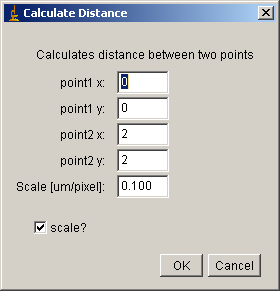
\includegraphics[scale=0.6]{fig/fig2421_GenDialog.png}
\caption{Custom Parameter Input Dialog}
\label{figGenericDialog}
\end{center}
\end{figure} 

Line 2 to 9 creates a dialog box that has multiple input boxes that looks like Fig. \ref{figGenericDialog}. 

\begin{itemize}
\item Line 3 defines the title of the dialog window. 


\item Line 4 texts will be shown within the window. 

\item Line 5 to 11 defines the parameter input fields. Fields appear in the dialog box in the order of lines with Dialog.addNumber function in the macro. When you press OK button in the dialog box, parameter will be stored in the same order. 

\item Line 15 to 19 These values then are assigned to each variable by Dialog.getNumber(). 

\item Line 20 Checkbox is independent from these number fields and the value is returned by \ilcom{Dialog.getCheckbox()}. When you check the check box, the return value is 1. If not, the return value is 0. We use this Boolean value (true or false)  to decide if the scale will be multiplied to the distance [pixel] in Line 24.

\item Line 24 This if-statement does not have braces. Such simplification is possible if there is one line when "if" is true.  
\end{itemize}

You may also realize that the if statement in line 24 (and also in Line 28) does not have comparison like == or <  or so on. This is because \ilcom{switchscale} takes only 0 or 1 (\textbf{boolean}), which are interpreted as true ( \ilcom{switchscale} = 1) or false ( \ilcom{switchscale} = 0). So even without comparison, \ilcom{switchscale} is already a decision.  

\begin{indentexercise}{1}
Modify Code 5 so that two parameters are asked in a single dialog box. 
\end{indentexercise}
